\section{Introduction}

Large language model platforms must adapt one backbone to different tasks and resource limits. Parameter-efficient fine-tuning (PEFT) reduces adaptation cost by updating only a small set of model parameters, allowing a platform to maintain a \emph{registry} of configurations that differ in method, trainable modules, capacity, or training recipe. These trainable parameters determine a configuration's \emph{trainable subspace}: the update directions available during fine-tuning. Each training example can affect the model only through the directions that the target configuration exposes. Data selection reduces cost along a complementary axis by choosing a compact subset whose examples produce useful task updates. Its decisions therefore depend on the target trainable subspace: changing the subspace can change which examples the selector should prioritize.

Most data selectors ignore this interaction. Quality filters, diversity heuristics, and proxy-model scores produce one ranking for a task and reuse it across PEFT configurations. We call such a ranking \emph{PEFT-agnostic} because the selector does not receive the target configuration. Yet common PEFT methods permit different updates: LoRA adds low-rank changes to selected projections~\cite{hu2022lora}; adapters insert trainable bottlenecks~\cite{houlsby2019adapters}; and (IA)$^3$ scales selected activations~\cite{liu2022ia3}. The same example can therefore produce different updates, and hence have different value, under different configurations.

Gradient-based selectors capture this dependence but incur repeated computation. LESS~\cite{xia2024less} first builds a target-specific \emph{gradient datastore}, a cache containing a training gradient for each candidate example. It then ranks the candidates against a \emph{task sketch}, a small set of training or development examples that represents the target task. Because each PEFT configuration exposes different trainable parameters, LESS must rebuild the cache for every configuration. Its selection cost therefore grows linearly with the registry.

One shortcut is to reuse a single LESS subset for every configuration. This reuse avoids repeated computation but removes the configuration information that makes gradient selection useful. In our evaluation, the shortcut performs worse than a PEFT-agnostic representation baseline (Table~\ref{tab:quality-cost-headline}). Existing methods thus force a choice: recompute a target-specific ranking for every configuration or reuse a ranking that ignores the configuration.

\begin{figure*}[t]
\centering
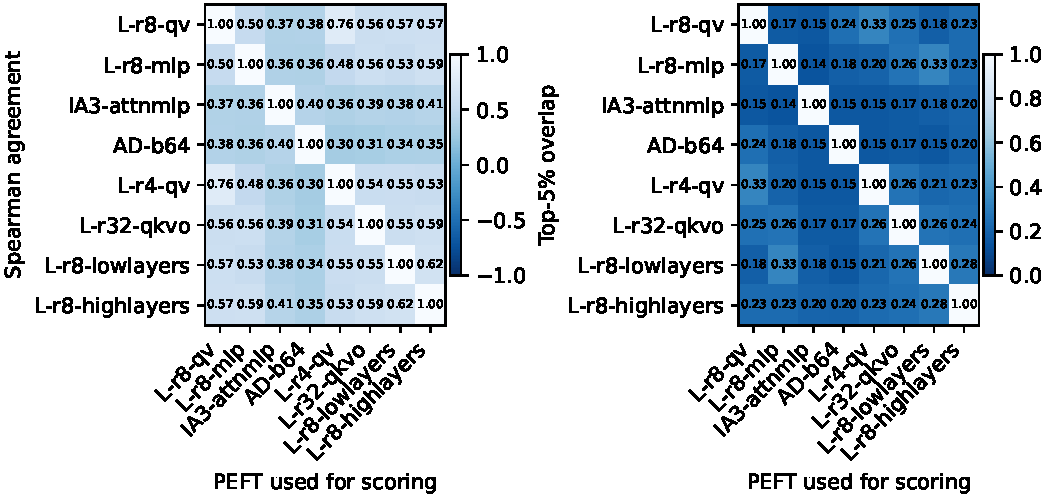
\includegraphics[width=\textwidth]{Figures/fig_motivation_disagreement.pdf}
\caption{Left: Spearman rank agreement between PEFT-conditioned utility rankings. Right: Top-5\% overlap between the corresponding selected examples; lower off-diagonal values indicate stronger configuration dependence.}
\label{fig:motivation-disagreement}
\end{figure*}

The configuration dependence affects downstream performance as well as the rankings. Figure~\ref{fig:motivation-disagreement} shows that independent runs for the same configuration agree more closely than runs across configurations. Changes within one PEFT family preserve more of the ranking, while cross-family changes produce the largest disagreement. Matched selection improves performance by 2.0 points over cross-family reuse and by 1.45 points within LoRA configurations (Supplementary Table~S10 and Figure~S1).

These observations motivate \emph{PEFT-conditioned utility}: the value of training on example $x$ for task $t$ under PEFT configuration $p$. We denote this value by $u(x,p,t)$. A task-only selector omits $p$ and must assign the same ranking to every configuration. Per-PEFT influence selection includes $p$ but recomputes gradients for each target. Our goal is to predict $u(x,p,t)$ while sharing the expensive computations used to learn these scores.

PCU-Select (PEFT-Conditional Utility) enables this sharing through a common representation. It maps every supported configuration to 24 \emph{intervention sites}: selected Transformer module outputs through which PEFT updates affect the backbone. These outputs remain comparable even when PEFT methods train parameter tensors with different shapes. PCU-Select caches sample and task signals at the sites. A structured PEFT code records which sites a configuration affects, its update type, its capacity, and its training recipe. Supplying this code at scoring time preserves configuration information while keeping the cached signals reusable.

A conditional scorer turns the shared signals into a target-specific ranking. Its prediction depends on the candidate example, task sketch, and PEFT code. It learns from two complementary signals: inexpensive labels based on gradient alignment cover the full candidate pool, while short-update labels measure task-sketch loss reductions for a smaller sample. At deployment, the scorer ranks the cached examples for a target configuration and task. PCU-Select then spreads the budget across groups of semantically similar examples to limit near-duplicates. This pipeline moves gradient extraction and label construction offline while retaining a distinct subset for each target.

These design choices amortize target-specific selection across a PEFT registry. We make three contributions:
\begin{itemize}
    \item \textbf{PEFT-conditioned utility.} We define data value as a candidate example's usefulness for a given task and PEFT configuration. We show that both rankings and downstream subset quality change with the target configuration.
    \item \textbf{Intervention-site amortization.} PCU-Select maps different PEFT parameterizations to 24 shared module-output sites. A structured code retains each target's update structure and recipe, enabling configuration-specific rankings without rebuilding gradient datastores; ablations validate both PEFT and task conditioning.
    \item \textbf{Registry-scale quality and cost.} Across four tasks and five seen PEFTs on Llama-2-7B~\cite{touvron2023llama2}, PCU-Select gains 0.74 points over RDS+ and matches per-PEFT LESS within $+0.04$, while cutting four-task PEFT onboarding by $42\times$, from 63.2 to 1.51 GPU-hours.
\end{itemize}
